\chapter{Concurrency Control}
\minitoc

This chapter is about concurrency control...  \\

We shall describe the result of the mutual exclusion exercise. In section \ref{MutualExclusion_solution} we demonstrate our solution. In section \ref{MutualExclusion_run} we show an example run of the solution. In section \ref{MutualExclusion_motivation} we discuss the underlying theory and relate that to the solution. In section \ref{MutualExclusion_conclusion} we round up the chapter.

\section{lab description}
\textit{The main objective of this week’s assignment is to understand some of the primary challenges of concurrency control. In order to understand those challenges, we will use Task Manager group communication, bulding on the last week’s lab exercise using JGroups.}\\

\textit{The sample code is provided in order to help you to understand how a task can results into different states if it is executed concurrently at different task manager servers. This week’s sample code is more or less similar to the last week’s sample code and uses JGroups for group communication among the Task manager servers. Even though each task manger uses a individual task manager Xml file, the tasks in the xml files are the same. It offers two simple operations on the tasks as described below.}

\begin{itemize}
\item \textit{\textbf{execute:} accepts id of a task and executes the task by assigning the ’status’ attribute to ‘executed’ and ‘required’ attribute to ‘false’. After the execution of the task, the task manager server will inform all other task manager servers in the group to execute the task matching to id.}
\item \textit{\textbf{request:} accepts id of a task and assigns the ‘required’ attribute to ‘true’ for the task matching to the id. Then, the task manager server will inform to all other task manager servers in the group for making the same changes to the task at their respective locations.}
\end{itemize}

\textit{The basic idea is to initiate to ‘execute’ and ‘request’ operations on a task with same Id from two different instances of task manager concurrently. If these operations are carried out concurrently at different task manager servers, then the task would results in different states based on the sequence of two operations carried out at the respective task manger servers.  For example, at one task manager, if ‘execute’ is followed by ‘request’, then the final state of task will set the attribute required=’true’, on the other hand at an another task manger server, if the ‘request’ followed by ‘execute’ then the task will have the attribute required=’false’.}\\

\textit{\textbf{The Assignment}\newline As part of the this week’s assignment, your task is to Implement a mutual exclusion algorithm (as explained in chapter 15 of DS text book) protecting the change of state of a task. Furthermore, analyze your  mutual exclusion algorithm for:}

\begin{itemize}
\item \textit{Safety (ME1)}
\item \textit{Liveness (ME2)}
\item \textit{Ordering(ME3) [optional]}
\end{itemize}

\textit{as described on page 650 of DS text book. You should also try to evaluate the performance of your mutual exclusion algorithm according to the criteria specified on page 651 of DS text book (bandwith, client delay and synchronization delay).}

\section{Solution}
\label{MutualExclusion_solution}
The soultion to this assignment is primarily based on the solution of the former chapter, Indirect Communication, where there are two primary classes for solving this assignment; TaskManagerServer and TaskReceiver2. \\

The TaskManagerServer´s primary function in the relationship between two the classes, is to send request to other TaskManagerServer´s, while TaskReceiver2 receives the requests on behalf of the TaskManagerServer´s and executes them. \\

The solution uses the same JGroup system for sending and receiving messages, so this chapter will not so much focus on the setup of the two classes, but rather the process of how requests are handled in this mutual exclusion solution, which uses the simple concurrency control protocol as described on the blog: \url{https://blog.itu.dk/SMDS-E2013/schedule/lab-exercise-07/} \\

The General idea of the simple concurrency control protocol is; that each Server must be able to lock the tasks which they wish to execute, send a request to all other servers and wait until it has been given authorization to execute the task. \\

In order for the Server´s to be able to lock the tasks they wish to execute, each Server has a hashtable wich contains the taskId as key and then the amount of Grantlocks it needs, which is the number of members in the group -1, before the task is executable, as value. \\

When we need to process the requests and execute the tasks we are in need of 4 different tokens: RequestLock, GrantLock, DenyLock and Commit. We havent made the tokens, however we use strings which we pass around to the different receivers using the envelope. The envelope now contains two string fields; command and lock, in order to tell the receiver what to do. \\

When a Server wants to execute or request a task, it first checks if it already has the task listed in its hashtable. If the the task is already there, then the user will be informed that the task is already enlisted. Else we add the task to Server´s own hashtable with the number of grantlocks needed, and then sends a request to all the other members of the group. \\

When the group members receives a request they first check if they have the task enlisted in their own hashtable. If they do not have the task enlisted, then they will send back a grantlock back to the server which requested it. If the server infact do have the task inlisted in its hashtable then it will send a denylock back to the requesting server. \\

If the server receives a denylock it will imediately delete the specified task from the hashtable. However if the server receives a grantlock, then it will countdown the number of grantlocks needed for the specific task, and if the countdown hits zero, then the server sends a Commit to all members of the qroup. \\

When a Server is given a Commit, it will execute the command on the specified task and save its xml-file. And thus is the simple concurrency control implemented. \\

We ran into some troubles concerning how to send a message to only one member of the group. There where also some degree of confusion as when to send a message to one or all members of the group. \\


\section{Example Run}
\label{MutualExclusion_run}

In this run we will run 3 TaskManagerServers each with its own xml task file. After the servers has been initialized we will ask two of the servers to do an execute and a request operation on the same task, and then hopefully one of them will be able to run its command, while the other will be denied. \\

%\begin{center}
%\centering
\caption{Server 1}
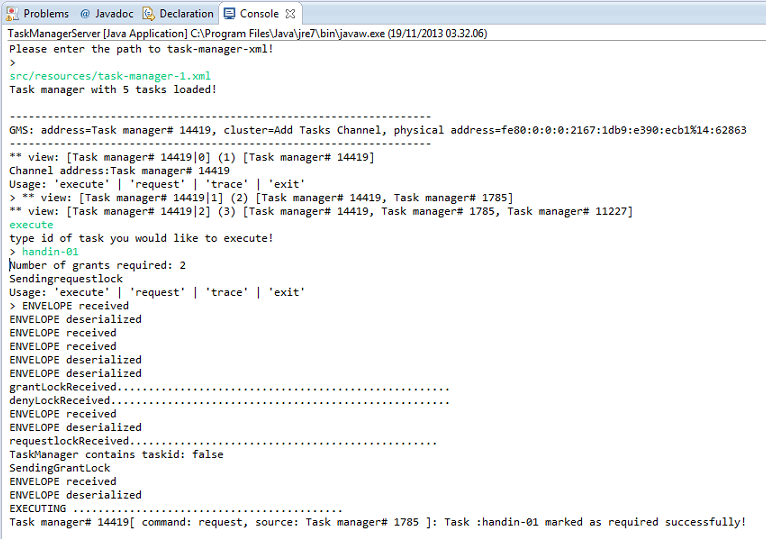
\includegraphics[scale=0.6]{images/CCServer1.png}
%\end{center}
%\vspace{10pt}

In the first server we run the execute command. The server sends a request to the other servers and receives a grantlock from server 3, which is not running any commands, and a denylock from server 3, which is running the request command. After receiving the denylock, the server then deques the task and wait for new orders. Then after a while the server is asked for grantlock from server 2 which it gives, because it no longer has the task in the hashtable. After that it then receives a commit from server 2, and performs the request command on the specified task. \\

%\begin{center}
%\centering
\caption{Server 2}
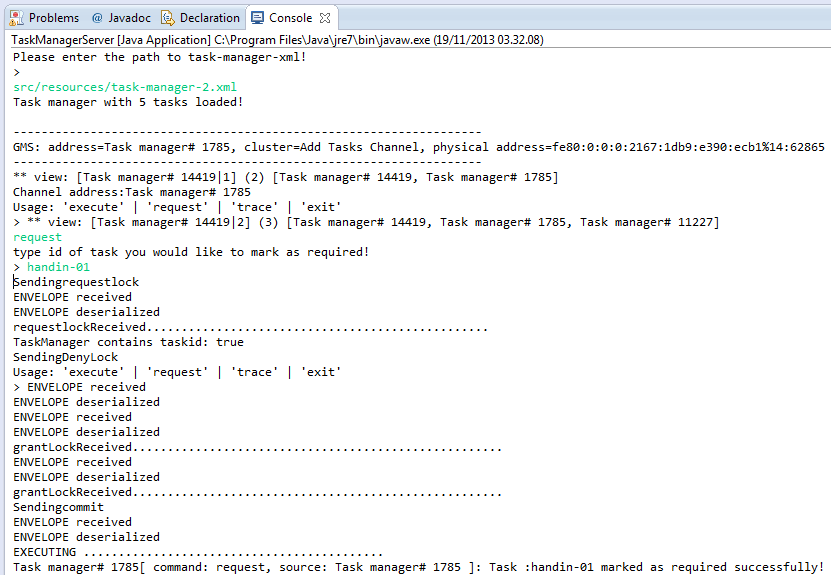
\includegraphics[scale=0.6]{images/CCServer2.png}
%\end{center}
%\vspace{10pt}

In the second server we run the request command. The server send a requestlock to the other servers, but before it receives any feedback, it gets a request from server 1 and since server to has the same task in the hashtable it sends back a denylock. After sending the denylock, it receives a grantlock from both servers, and then because the requirement for grantlocks is forfilled, it sends a commit to all servers including itself, telling them to execute its command on the specified task. \\

%\begin{center}
%\centering
\caption{Server 3}
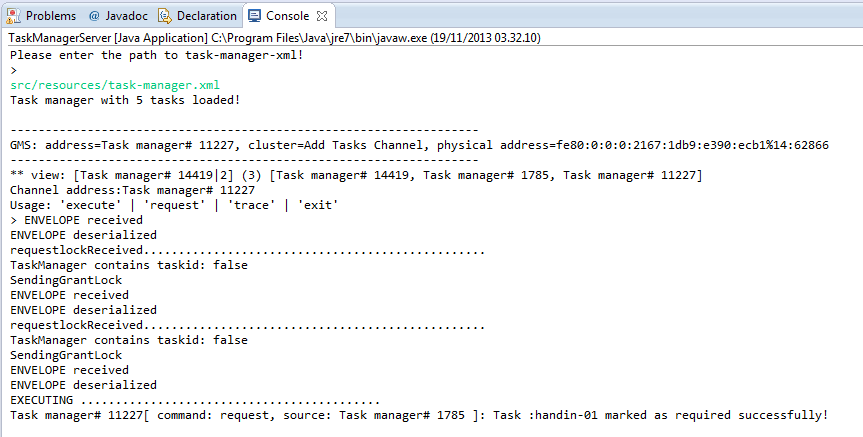
\includegraphics[scale=0.6]{images/CCServer3.png}
%\end{center}
%\vspace{10pt}

in the third server no command is run. The server receives a requestlock from the other servers and since it doesnt have any commands running, it simply sends back a grantlock. After a while it then receives a commit from server 2 and performs the command on the specfied task. \\

We sometimes run into the problem, that two servers might both get a denylock, if they send the requestlock on the same time. This means that no command will be run on the specified task, which is undesireable. The problem can be solved using timestamps.

\section{Motivation- and theory}
\label{MutualExclusion_motivation}

\subsection{Coordination: Mututal Exclusion}
Mututal exclusion algorithms are used in systems where there is some common resources, which are accessed from several different users eg. servers. The algorithms for distributed mutual exclusion rely on message passing which can either be; permission based or token based. \\

For all distributed algorithms there are the following requirements:
\begin{itemize}
\item \textbf{ME1:} At most one node may be in the critical section at a time (Safety)
\item \textbf{ME2:} Requests to enter/exit eventually succeed 
(liveness)
\item \textbf{Optional ME3:} Requests are served in happened-before 
order (ordering)
\end{itemize} 

Following the requirements there is also a set of mutex quality measurements:
\begin{itemize}
\item \textbf{Bandwidth:} messages per entry/exit
\item \textbf{Client delay:} messages required for entry+exit
\item \textbf{Synchronisation delay:} messages required from resource is exited, until it is next entered
\end{itemize}

There are several different ways to make a permission based mutual exclussion. It can be:
\begin{itemize}
\item \textbf{Centralised:} A single coordinator handles entry.
\item \textbf{Decentralised:} A majority of coordinators must say ok before entry.
\item \textbf{Distributed:} Everyone must say ok before entry. 
\end{itemize}  

One of the more prominent token based algorithms is:
\begin{itemize}
\item \textbf{Token Ring:} A token is constantly based around when a node needs the token it, accesses it, when it gets it, and passing it on when releasing it. 
\end{itemize} 

There are also other mutual exclussion algorithms, which are based on elections, which are very good at handling crashes. \\

The simple concurrency control protocol. which we used to make this assignment, is most similar to ditributed permission, as the node needs permission from all other nodes. Though they are very similar, the concurrency control lacks in some areas. \\

\textbf{Fulfilling requirements:}
\begin{itemize} 
\item \textbf{ME1(Safety):} Since all nodes must give a granLock before a node may enter the critical section, it is pretty certain to say that it is save. 
\item \textbf{ME2 (Liveness):} In terms of Deadlock we are certain that only one Node is capable of entering the critical state so there should be no problems in exiting the critical state. However when a Node requests permission from the other nodes and one of the nodes crashes, then that node will never be able enter the critical state, and all other nodes will be prevented from entering, which is a clear deadlock! In terms of starvation the concurrency control is also very poor. When a node is given a denylock, the operation is simply removed, which means that it will never be executed. That problem leads to ultimate starvation. Also because of this, the concurency control isn´t fair either, and doesnt even pass the other fairness requirement, which is happened-before ordering, which is also stated in the run.
\item \textbf{ME2 (Ordering):} As stated in Liveness the concurrency control doesnt support happened-before ordering.
\end{itemize}

\textbf{Quality of the simple concurrency control protocol:}
\begin{itemize}
\item \textbf{Bandwidth:} The concurrency control uses 3(n-1) messages to enter and exit the critical stat. First have to send requests to all other nodes, then all the nodes receiving the requests has to send back a reply, and finally when the operation is going to be executed, the node again has to send a message to all the other nodes, in order for them to executing operation as well. This is terribly slow!
\item \textbf{Client delay:} In terms of client delay the concurrency control again uses 3(n-1).
\item \textbf{Synchronisation delay:} Since the concurrency control has not implemented the option to queue operation requests, but just sends denylock, which ensures that the request is terminated, then the time for a the resource to be entered into CS again will take 2(n-1). Which again states how bad this system is!
\end{itemize}

\section{Conclusion}
\label{MutualExclusion_conclusion}
We have implemented the simple concurrency control protocol as described in the assignment description, with one deviation being that we use strings instead of tokens. The SCCP successfully satisy the requirements of the assignment, however there are many drawbacks to the chosen soloution. The first problem we run into is the deadlock, where one node waits for a request from a crashed node. In terms of livenes and ordering it would be pretty simple to implement a queue of requests for each node, and to add a timestample to the requests, which would fix the problems with starvation and ordering. The queue would also inprove the Synchronisation delay from 2(n-1) to 1.
So to sum up; the solution meets the requiremnts, but could certainly be better!
